\documentclass{article}
\usepackage{graphicx}
\title{Tetrahedronized Boundary Layer Refinement}
\author{Dan Ibanez}
\date{May 17, 2014}
\begin{document}
\maketitle

This document explains the issue with uniform refinement
of a tetrahedronized boundary layer, i.e. how it does not
preserve the stack structure of the boundary layer.

First we must understand the uniform refinement template
for a tetrahedron. In this case, all edges have been split,
each of the original triangular faces have been split into four
new faces, and we are left with the problem of tetrahedronizing
the interior. The following figure illustrates this template:

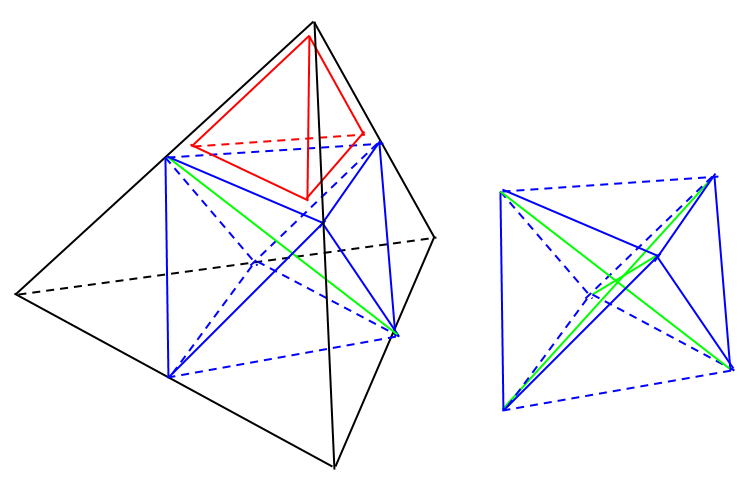
\includegraphics[width=0.8\textwidth]{tet_uniform_refine.png}

In this figure, the original tet is black, and the new blue edges are
determined when splitting the faces.
The first thing we do is to create four sub-tetrahedra in the corners.
One of these is highlighted in red for clarity.
After these sub-tets are created, we are left with the central blue cavity
which is octahedral.

This cavity is filled with 4 tets by choosing one of 3 possible diagonal
edges and creating tets around it.
This is preferrable in several ways to creating a central vertex.
The figure extracts the octahedral sub-volume and shows in green the three
possible diagonals.
The tet is shown refined using one of these diagonals.
Note that the choice of diagonal is made based on shortest length in metric
space.

Now we can show how the unrestricted choice of diagonal can cause a problem
if we try to refine a boundary layer represented as tetrahedra instead of
prisms.
The following figure shows a ``prism" composed of tetrahedra being uniformly
refined:

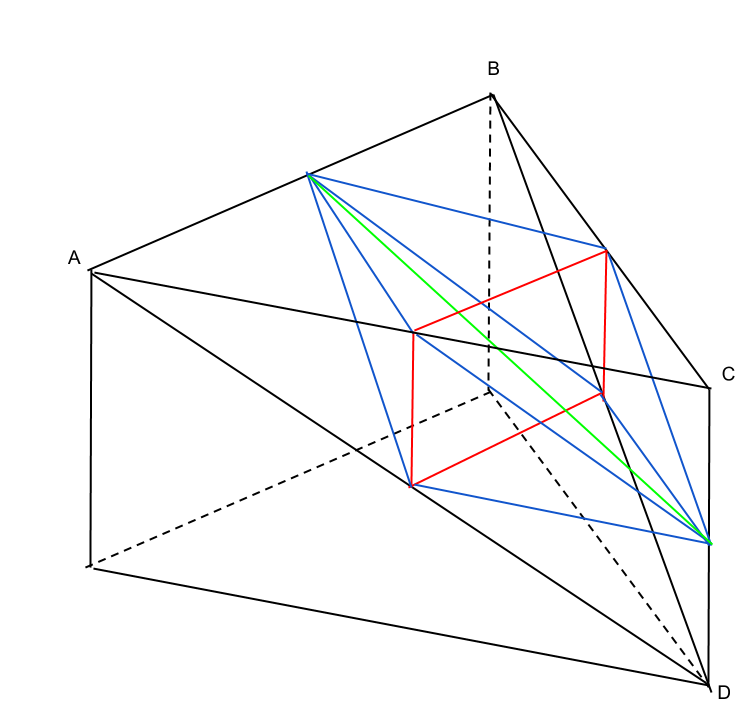
\includegraphics[width=0.8\textwidth]{prism_uniform_refine.png}

The ``prism" is colored black and the tet of interest (ABCD) is also outlined in black.
For now take it for granted that tetrahedronization will always produce one
tet such as this one for each prism, how that happens is for another document.
Now note the tet being uniformly refined.
Its octahedral sub-volume is again outlined in blue, but this time we focus
on one ring of edges in it that looks like a quad, outlined in red.
Looking at the overall prism, we would expect this red ``quad" to become a face
(or two triangular faces at least), since the boundary layer stack is being
subdivided into four adjacent stacks and that ``quad" separates two of the refined
stacks.

Unfortunately, there is one diagonal choice that will break through the ``quad"
and violate the structure of the boundary layer stack.
While it may be an unlikely choice given our metric space heuristic, we cannot
rely on that to preserve structure.
Introducing artifical constraints on tetrahedral refinement also seems like
the wrong way to go.

This one of the reasons why we want to perform all adaptation of
the boundary layer using a mixed mesh representation and tetrahedronize only
after this adaptation is done and the mesh is ready for analysis.

\end{document}
